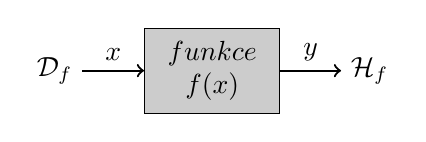
\begin{tikzpicture}[fill=black!20]
%  \draw[help lines] (-1,-2) grid (6,3);
  \path (0,0) node(a) [ ] {\(\mathcal{D}_f\)}
  (2,0) node(b) [rectangle,rotate=0,draw,fill] {\(\begin{array}{c} \text{funkce} \\ f(x)  \end{array}\)}
  (4,0) node(c) [ ] {\(\mathcal{H}_f\)};
  \draw[thick,->] (a.east) -- (b);
  \draw[thick,->] (b.east) -- (c);
  \path [ ] (a.east) -- (b.west)   node [above,midway] {\(x\)};
  \path [ ] (b.east) -- (c.west)   node [above,midway] {\(y\)};
\end{tikzpicture}